\documentclass[12pt]{article}
 
\usepackage[margin=.5in]{geometry} 
\usepackage{amsmath,amsthm,amssymb,outlines}
\usepackage{graphicx,tikzsymbols,tcolorbox, bbm}
\renewcommand\qedsymbol{$\blacksquare$}
\newcommand{\Z}{\mathbb{Z}}
\newcommand{\R}{\mathbb{R}}
\newcommand{\doublearrow}[1]{\xrightarrow[]{#1}\mathrel{\mkern-14mu}\rightarrow}
\tcbuselibrary{most}

\newtcolorbox{newtitle}{
  enhanced,
  colframe=black,
  colback=white,
  boxsep=5pt,
  arc=8pt,
  sharp corners=south,
  borderline={0.5pt}{0pt}{black},
  borderline={1.8pt}{-5pt}{black},
  after skip=30pt
}

\newtcolorbox[auto counter]{statement}[1][]{
  enhanced,
  breakable,
  title={Exercise \ifx\\#1\\\thetcbcounter\else#1\fi},
  colframe=black,
  colback=white,
  colbacktitle=white,
  fonttitle=\bfseries,
  coltitle=black,
  attach boxed title to top left={yshift=-0.25mm-\tcboxedtitleheight/2,yshifttext=2mm-\tcboxedtitleheight/2, xshift=2mm},
  boxed title style={boxrule=0.5mm}
}

\newtcolorbox{newproof}{
  enhanced,
  breakable,
  frame hidden,
  colback=white,
  title={Proof.},
  fonttitle=\bfseries,
  coltitle=black,
  colbacktitle=white,
  boxed title style={boxrule=0.5mm},
  attach boxed title to top left={yshift=-0.25mm-\tcboxedtitleheight/2,yshifttext=2mm-\tcboxedtitleheight/2, xshift=2mm},
  borderline west={1.5pt}{8pt}{black},
  after upper={\hfill $\blacksquare$}
}

\begin{document}

\begin{newtitle}
  \begin{center}
    \textbf{\Huge 8200 Homework 11}
  \end{center}
  \textbf{} \hfill \textbf{\today}
\end{newtitle}

\begin{statement}[2.2.22]
    For $X$ a finite CW complex and $p : \widetilde{X} \to X$ an $n$-sheeted covering space, show that $ \chi(\widetilde{X}) = n \chi(X). $
\end{statement}
\begin{newproof}
    The Euler characteristic is an alternating sum of the cells in the CW Complex
    $$ \chi(X) = \sum^{\infty}_{k=0} (-1)^k c_k $$
    where $c_k$ is the number of $k$-cells in $X$. In any covering space, each $k$-cell in the CW complex must be covered the same amount of times, and this is what gives us our number of sheets. So in an $n$-sheeted covering space, there are $n \cdot c_k$ $k$-cells. Thus
    $$ \chi(\tilde{X}) = \sum^{\infty}_{k=0} (-1)^k n \cdot c_k = n \sum^{\infty}_{k=0} (-1)^k c_k = n \chi(X).$$
\end{newproof}

\begin{statement}[2.2.23]
    Show that if the closed orientable surface $M_g$ of genus $g$ is a covering space of $M_h$, then $ g = n(h - 1) + 1 $ for some $n$, namely, $n$ is the number of sheets in the covering. [Conversely, if $g = n(h - 1) + 1$ then there is an $n$-sheeted covering $M_g \to M_h$, as we saw in Example 1.41.]
\end{statement}
\begin{newproof}
    We know the Euler characteristic of an orientable surface is $\chi(M_g)=2-2g$ (or for $M_h$, $\chi(M_h)=2-2h$). From the previous problem, we know that if $n$ is the number of sheets in the covering, $\chi(M_g)= n \cdot \chi(M_h)$. So we are left with
    \begin{align*}
        2-2g &= n(2-2h) \\
        2-2g &= 2n -2nh \\
        1-g &= n - nh \\
        -g &= n -nh - 1 \\
        g &= nh - n + 1 \\
        g &= n(h-1) + 1.
    \end{align*}
\end{newproof}

\begin{statement}[2.2.28]
    \begin{itemize}
        \item[(a)] Use the Mayer–Vietoris sequence to compute the homology groups of the space obtained from a torus $S^1 \times S^1$ by attaching a Möbius band via a homeomorphism from the boundary circle of the Möbius band to the circle $S^1 \times \{x_0\}$ in the torus.

        \item[(b)] Do the same for the space obtained by attaching a Möbius band to $\mathbb{RP}^2$ via a homeomorphism of its boundary circle to the standard $\mathbb{RP}^1 \subset \mathbb{RP}^2$.
    \end{itemize}
\end{statement}

\begin{statement}[2.2.30]
    For the mapping torus $T_f$ of a map $f : X \to X$, we constructed in Example 2.48 a long exact sequence $ \cdots \to H_n(X) \xrightarrow{\mathbbm{1} - f_*} H_n(X) \to H_n(T_f) \to H_{n-1}(X) \to \cdots .$ Use this to compute the homology of the mapping tori of the following maps:
    \begin{itemize}
        \item[(a)] A reflection $S^2 \to S^2$.
        \item[(b)] A map $S^2 \to S^2$ of degree $2$.
        \item[(c)] The map $S^1 \times S^1 \to S^1 \times S^1$ that is the identity on one factor and a reflection on the other.
        \item[(d)] The map $S^1 \times S^1 \to S^1 \times S^1$ that is a reflection on each factor.
        \item[(e)] The map $S^1 \times S^1 \to S^1 \times S^1$ that interchanges the two factors and then reflects one of the factors.
    \end{itemize}
\end{statement}

\begin{statement}[1.2.9]
    In the surface $M_g$ of genus $g$, let $C$ be a circle that separates $M_g$ into two compact subsurfaces $M'_h$ and $M'_k$ obtained from the closed surfaces $M_h$ and $M_k$ by deleting an open disk from each. Show that $M'_h$ does not retract onto its boundary circle $C$, and hence $M_g$ does not retract onto $C$. [Hint: Abelianize $\pi_1$.] But show that $M_g$ \emph{does} retract onto the nonseparating circle $C'$ in the figure.
  \begin{center} 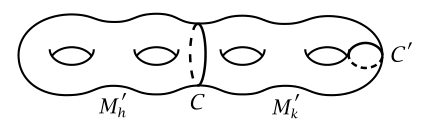
\includegraphics[scale=.8]{5.1.png} \end{center}
\end{statement}
\begin{newproof}
    First, we'll show that $M'_h$ does not retract onto its boundary circle $C$. For contradiction, assume that $M'_h$ does retract onto its boundary circle $C$ with $r: M'_h \to C$. Then there must exist $r_*:\pi_1(M'_h) \doublearrow{} \pi_1(C)$, but we know $\pi_1(C) \cong \Z$, so $r_*:\pi_1(M'_h) \doublearrow{} \Z$. We also know $\pi_1(M'_h)= \langle a_1,b_1, \dots, a_h, b_h, c \vert \prod_{i=1}^{h} [a_i, b_i]=c \rangle$, but after abelianizing, $H_1(M'_h) \cong \Z^{2h} \oplus \Z$. But $H_1(C) \cong \Z$, so that $M_h'$ cannot retract onto $C$.
    \par To show that $M_g$ does retract onto $C'$, we can imagine a cut along $C'$, then collapsing on a segment orthogonal to it, then regluing, so that it can deform onto $C'$. 
\end{newproof}

\begin{statement}[2.C.5]
    Let $M$ be a closed orientable surface embedded in $\mathbb{R}^3$ in such a way that reflection across a plane $P$ defines a homeomorphism $r : M \to M$ fixing $M \cap P$, a collection of circles. Is it possible to homotope $r$ to have no fixed points?
\end{statement}
\begin{newproof}
    We can find the Lefshetz number by noting that $H_0(M) \cong \Z$ with trace 1, $H_1(M) \cong \Z^{2g}$ with an unknown trace, call it $t$, and $H_2(M) \cong \Z$ with trace -1. So the Lefshetz number is $-t$, so it can be zero, but that doesn't guarantee the existence of such a homotopy. Because $r$ is a reflection and $M \cap P$ is fixed, these loops are not hull-homotopic, so that there must exist some fixed points. So no, it is not possible to homotope $r$ to have no fixed points. 
\end{newproof}

\begin{statement}[2.C.6]
    Do an even-genus analog of Example 2C.4 by replacing the central torus by a sphere, letting $f$ be a homeomorphism that restricts to the antipodal map on this sphere. 
\end{statement}

\end{document}
